\chapter{Test Setup}
\label{chap:\currfilebase}

In the experiments conducted for this thesis, thin cuboid specimens were put under compressive force in direction of their longest side. The force was introduced in form of Combined Loading Compression (CLC), i.e. the compressive force was introduced by both end- and shear-loading as shown in\autoref{fig:specimen_loads}. In the setup it was both possible to record the forcing and displacement as well 
The test setup used consists of
\begin{itemize}
    \item the specimen
    \item a fatigue test system introducing and measuring load and displacement
    \item a test fixture, introducing the load of the test system to the specimen
    \item a CCD camera setup with the camera itself, a lens, light sources mounted on tripods
    \item a PC with software installed that allows synced recording of the fatigue test system and the CCD camera
\end{itemize}
Fatigue test system instron 8801
Combined loading compression CLC test fixture
Testing fixture ASTM D6641

\section{Specimen}
\label{sec:specimen}

The material used in the experiments is a unidirectional carbon fibre composite, cured from thermoset prepregs\footnote{TC250 Resin System in unidirectional tape format} using vacuum bag and autoclave. The specimens where then shaped by water jet cutting the flat plate. An example cutting pattern is shown in \autoref{fig:specimen_plateA}.
The Specimens were cut out in different angles with regard to the fibre direction. These angles are equal to the off-axis angle to the main loading direction when one neglects positioning inaccuracies.

\begin{figure}[!ht]
    \centering
    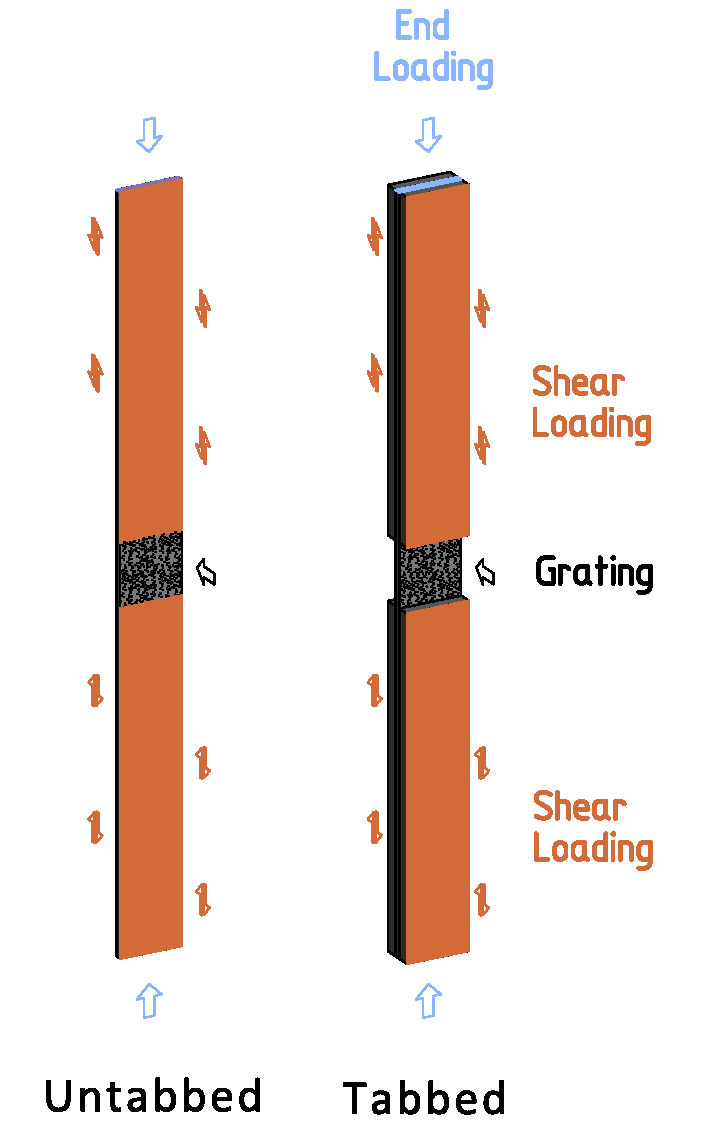
\includegraphics[scale=0.5]{\imgpath/\currfilebase/specimen_loads.pdf}
    \caption{Loads acting on both untabbed and tabbed specimens in setup respectively}
    \label{fig:specimen_loads}
\end{figure}
\begin{figure}[!ht]
    \centering
    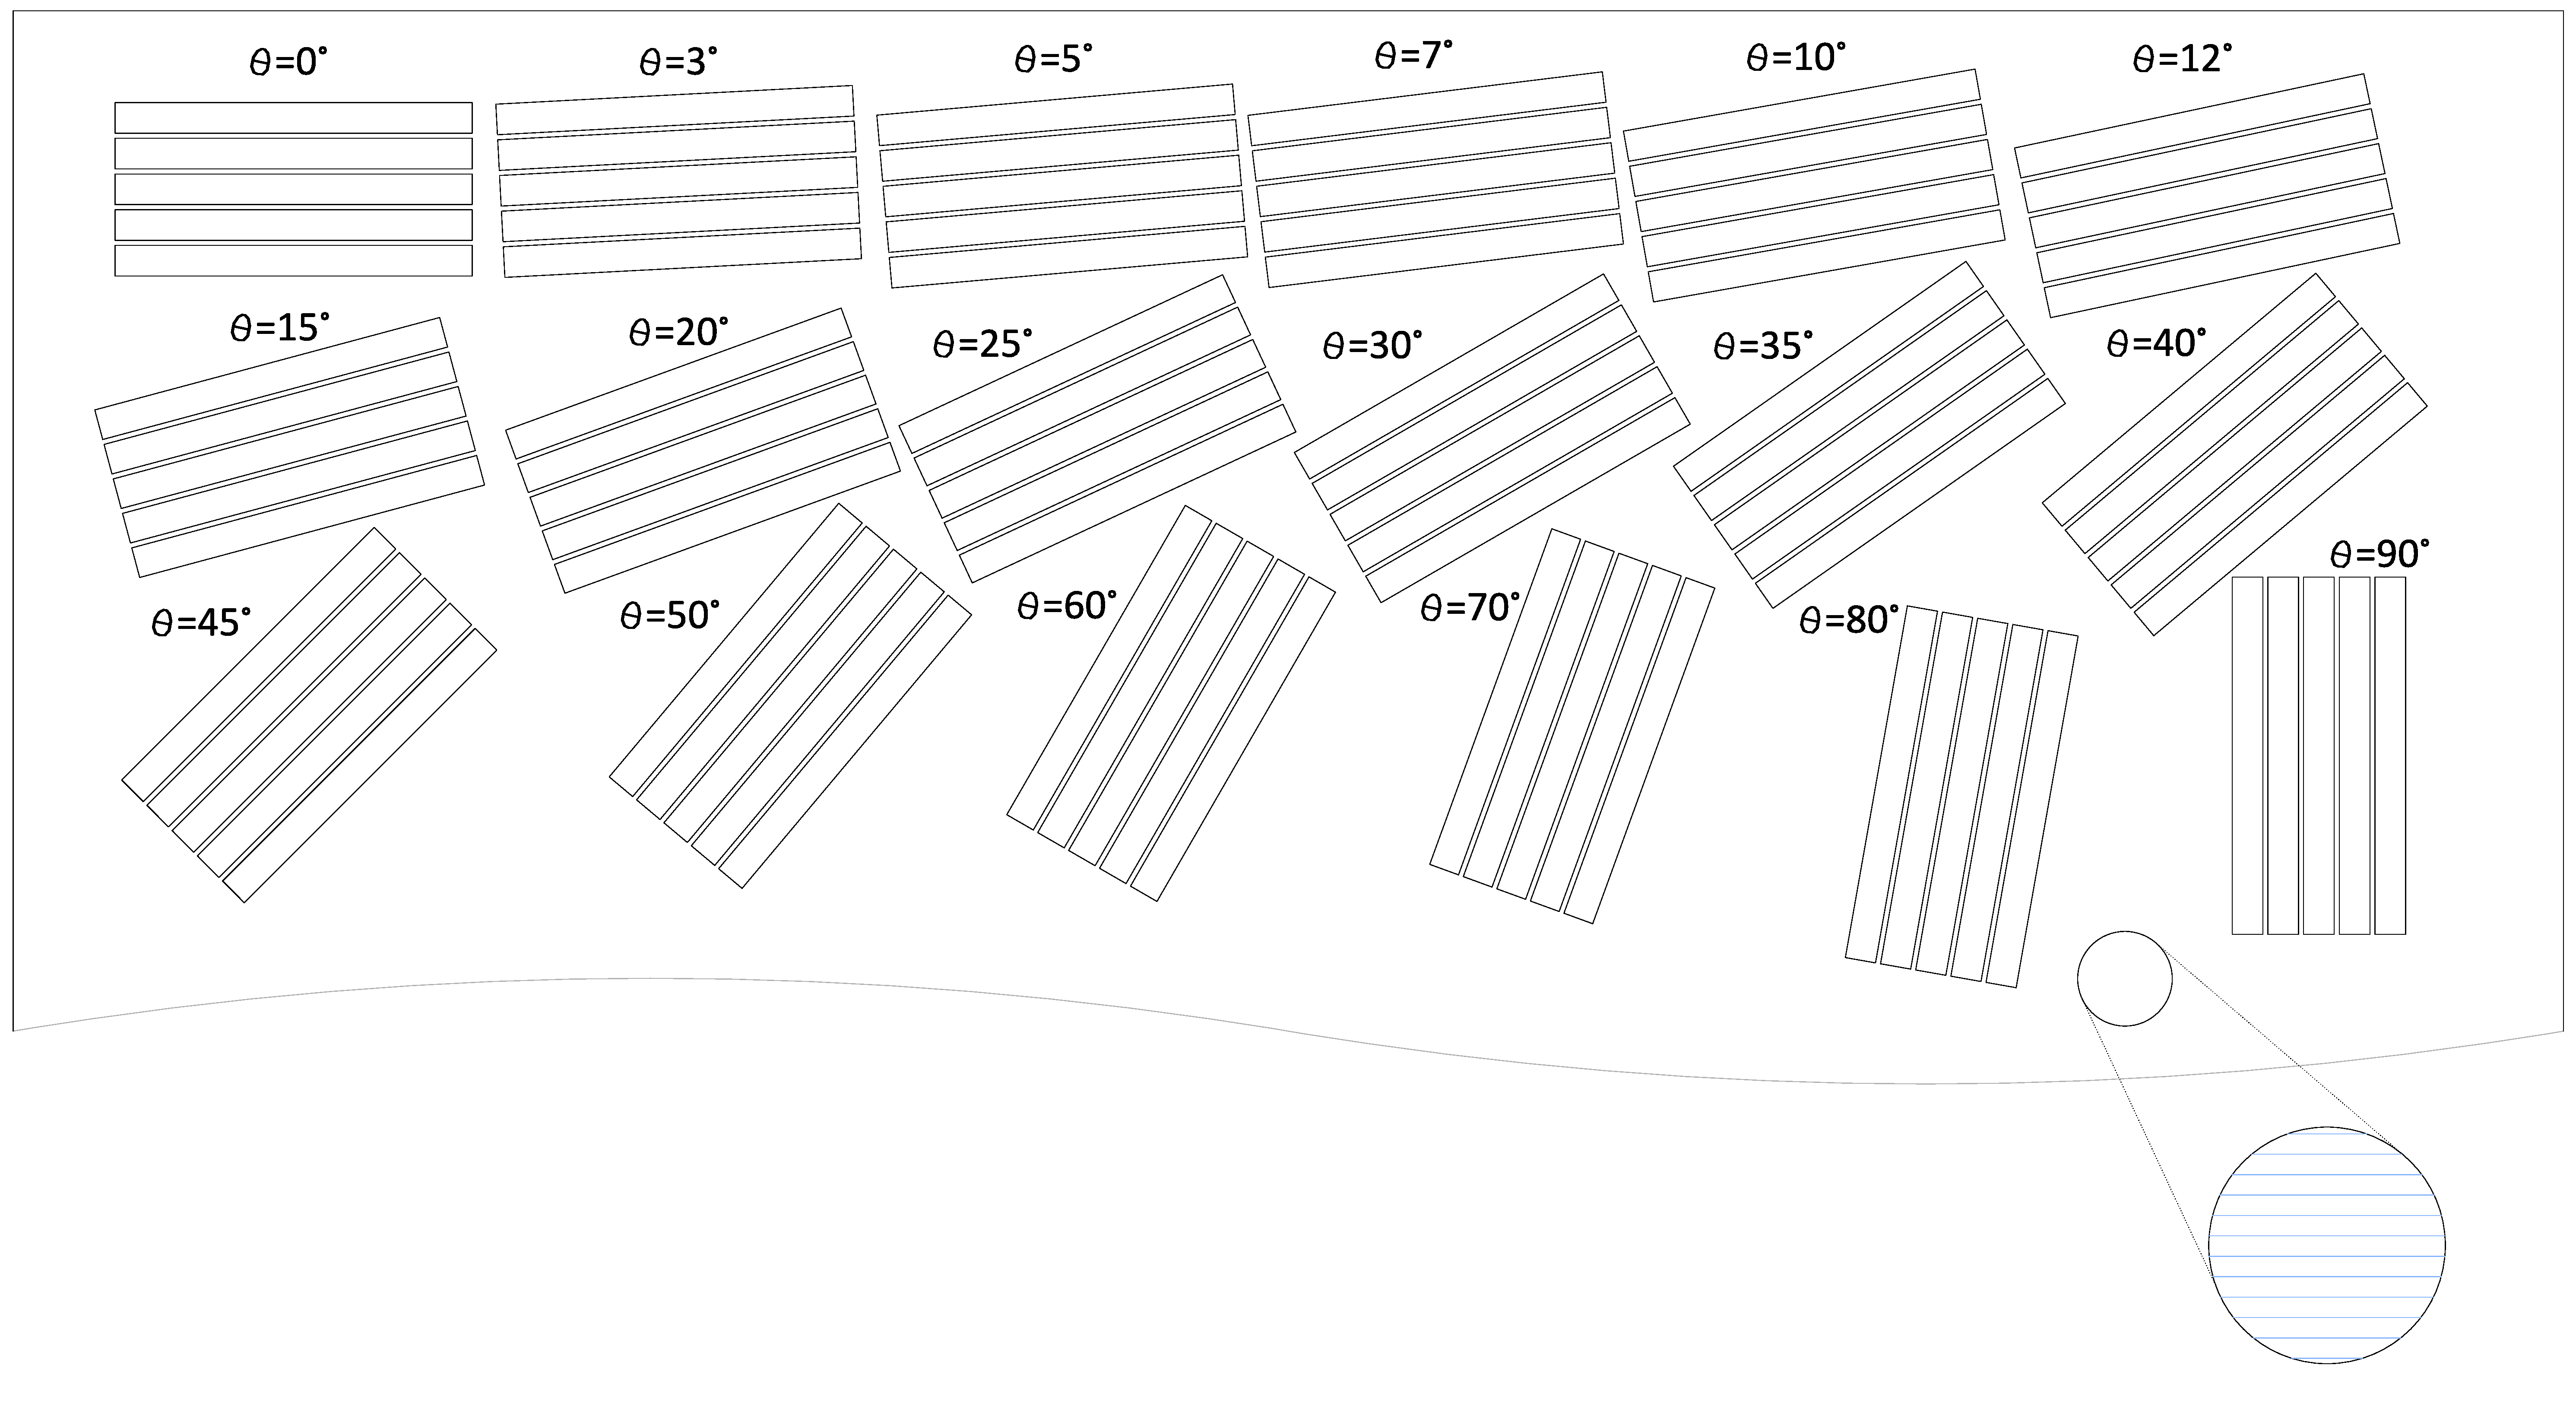
\includegraphics[scale=0.16]{\imgpath/\currfilebase/specimen_plateA.pdf}
    \caption{Water jet cutting pattern for carbon fibre plate with bottom right detail indicating the plate fibre direction}
    \label{fig:specimen_plateA}
\end{figure}
\begin{figure}[!ht]
    \centering
    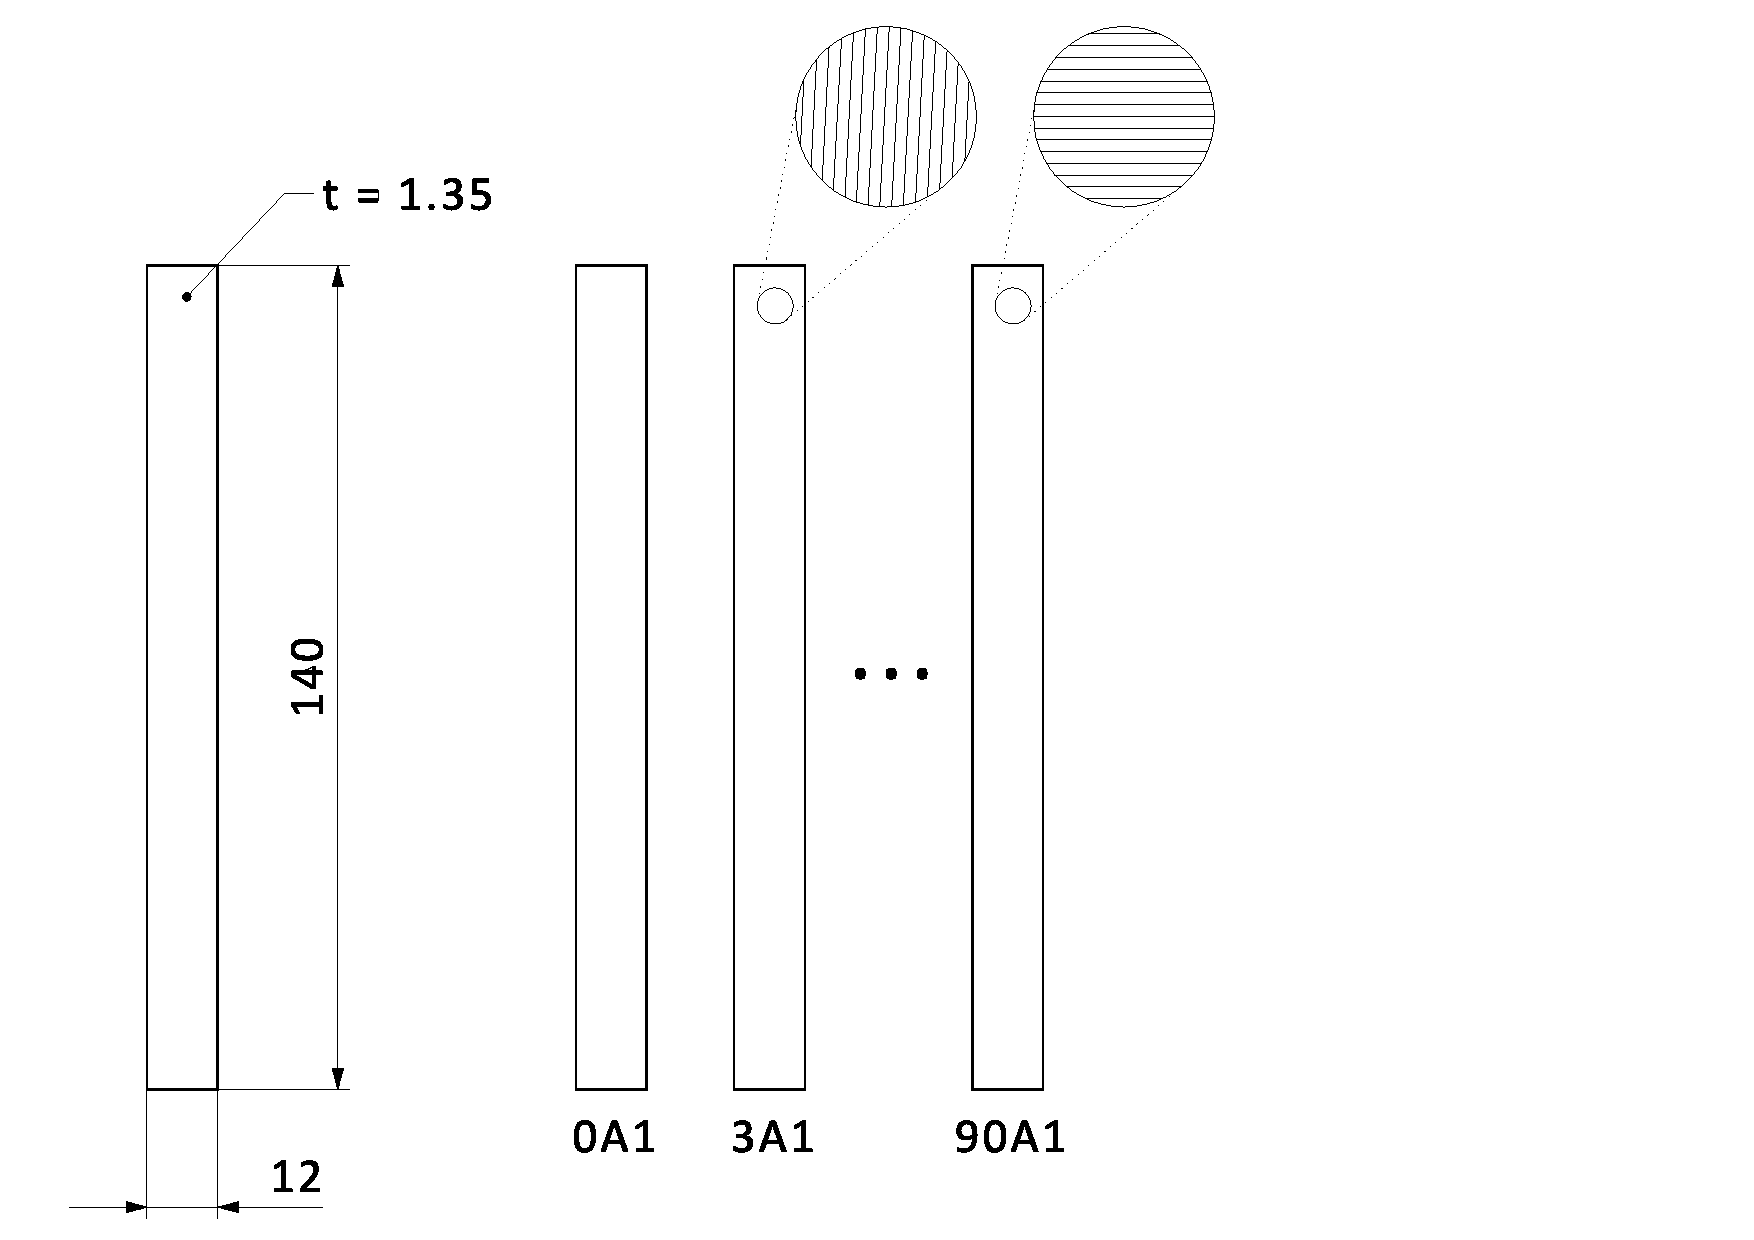
\includegraphics[scale=0.4]{\imgpath/\currfilebase/specimen_nx_dim_labels.pdf}
    \caption{Specimen dimensions and different fiber orientations}
    \label{fig:specimen_nx_dim_labels}
\end{figure}
\begin{figure}[!ht]
    \centering
    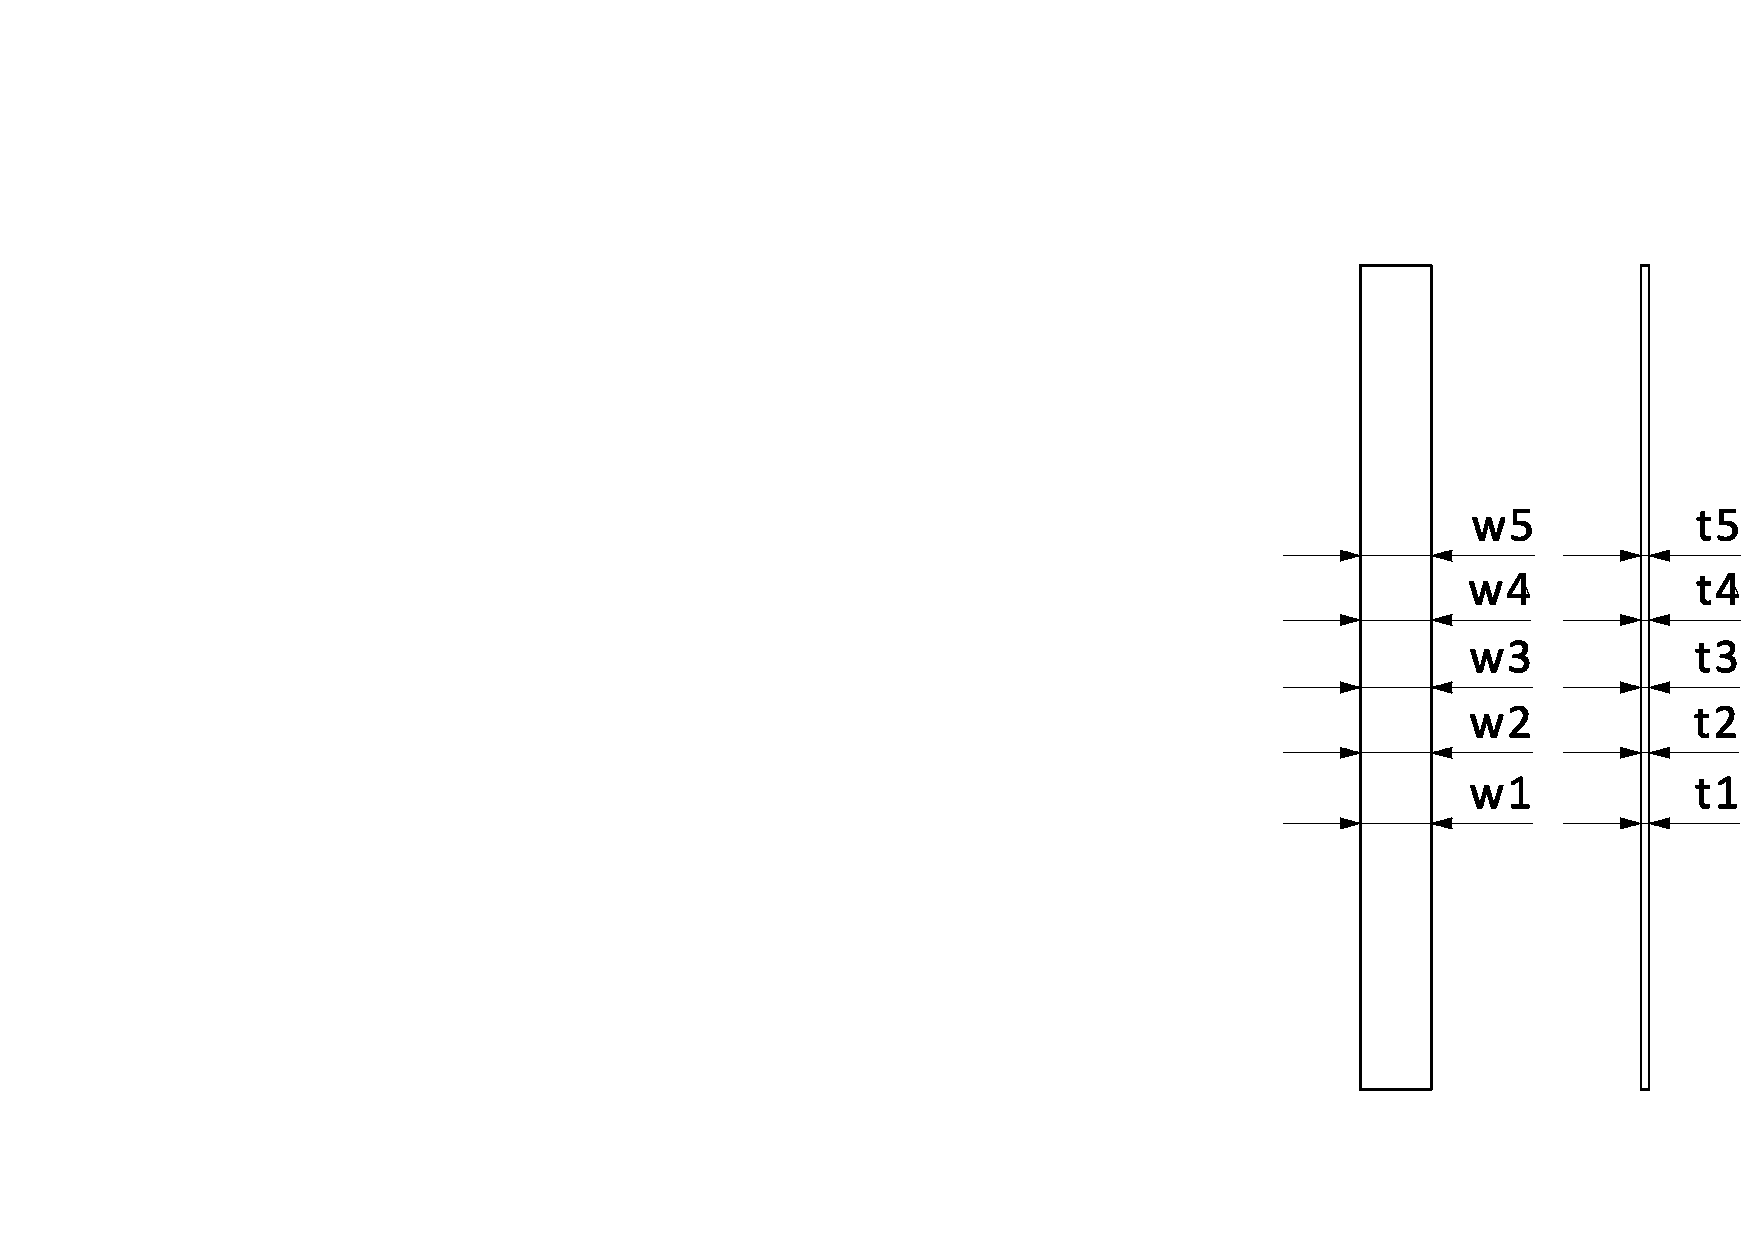
\includegraphics[scale=0.4]{\imgpath/\currfilebase/specimen_nx_meas.pdf}
    \caption{Specimen dimension measurements}
    \label{fig:specimen_nx_meas}
\end{figure}

\subsection{Specimen Preparation}
\label{sec:spec_prep}

\section{Fatigue Test System}
\label{sec:fatigue_test_sys}

\section{CCD Camera Setup}
\label{sec:ccd_cam_setup}

\section{Software}
\label{sec:software}


\section{Test Fixture}
The test fixture is a combined
\begin{figure}[!ht]
    \centering
    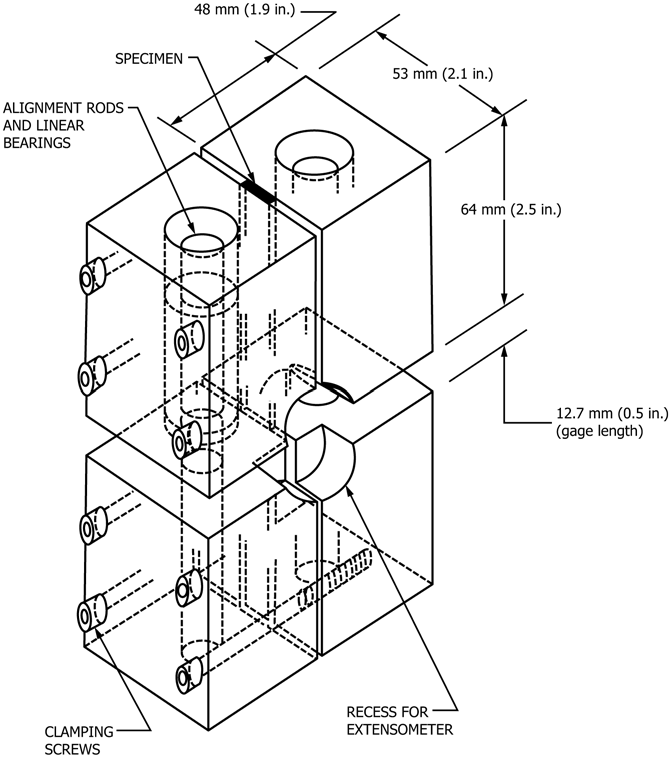
\includegraphics[scale=0.4]{\imgpath/\currfilebase/test_fixture.png}
    \caption{Dimensional Sketch of a Typical Combined Loading Compression (CLC) Test Fixture from \cite{D6641standard}}
    \label{fig:sketch_clc_fixture}
\end{figure}